\section{Baggrund}
For at undersøge sygdommen nærmere og øge forståelsen for de mekanismer der styre insulin reguleringen i kroppen laves der videnskabelige forsøg med Langerhanske øer.

De øer der anvendes til videnskabelige forsøg stammer typisk fra mus eller rotter. Sortering- og isoleringsprocessen foregår overordnet set ved 3 faser (\cite{per}), som vist i figur \ref{fig:sortproces}. 

\begin{figure}[H]
	\centering
	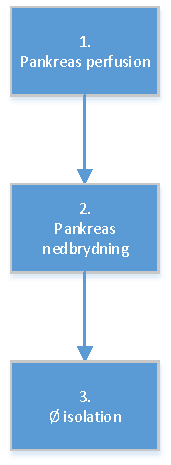
\includegraphics[width=0.2\textwidth]{billeder/sortering-crop.pdf}
	\caption{Faser i sorteringsprocessen}
	\label{fig:sortproces}
\end{figure}

Den første fase, \textit{pankreas perfusion}, foregår ved at  enzymet collagenase V sprøjtes ind gennem galdegangene og derfra videre til  pankreas. Dette enzym starter en nedbrydning af vævet i pankreas. Herefter fjernes pankreas operativt. Enzymet collagenase har den egenskab, at det ikke nedbryder de langerhanske øer i samme grad som det omkring liggende eksokrine væv.

I anden fase, \textit{pankreas nedbrydning}, nedbrydes pankreas yderligere ved, at inkubere pankreas ved 37° i 19 min. Ved denne temperatur er enzymet collagenase særligt aktivt og katalysere derfor nedbrydningen af pankreas. Herefter nedkøles vævet for, at stoppe virkningen af collagenase.

% sker derfor relativt hurtigt.  den bliver skåret i mindre dele og pankreas placeres i en inkubator ved 37,5 grader. Dette gøres for at accelerere nedbrydningen af pankreas. Når pankreas er nedbrudt nedkøles vævet for, at stoppe virkningen af collagenase. 

I den sidste fase, \textit{ø isolation}, vaskes og rystes øerne først af tre omgange med en vaskebuffer i form af en saltvandsopløsning (\cite{hbbs}). Dette gøres for, at løsrive øerne fra hinanden inden isolering. Herefter er øerne klar til at blive isoleret fra det eksokrine væv. Der findes en række forskellige metoder til dette, hvor den mest udbredte metode foregår ved manuel isolering af øerne fra en petriskål vha. et mikroskop. Der findes automatiserede isoleringsmetoder bygget på forskellige teknikker herunder gradient baseret centrifugering. Fælles for de anvendte teknikker til isolering af øerne er, at der er stor risiko for skade på øerne. 

Denne manuelle metode har yderligere ulemper i det, den både er besværlig og tidskrævende. Herudover kan der være stor variation i kvaliteten af isoleringen, da der kan være forskel på den enkelte operatørs håndtering af øerne. 

Derfor ønskes der en automatiseret metode til isolering af langerhanske øer, med minimal risiko for skader på øerne. En automatiseret metode vil have følgende følgende fordele \cite{pptintro}: 

\begin{itemize}
\item Øget sorteringshastighed for højere udbytte
\item Reducere variation i de isolerede øer
\item Reducere omkostningerne
\item Sikre bedre dokumentation
\item Forbedret arbejdsmiljø
\end{itemize} 

En automatiseret løsning vil potentielt åbne op for nye muligheder indenfor anvendelse af langerhanske øer. Der forskes bl.a. i transplantation af langerhanske øer, som et led i behandling af type 1 diabetes. Resultaterne af et af disse forskningsprojekter har bl.a. vist at 44 \% af modtagerne af denne type behandling var insulin uafhængige 3 år efter transplantation (\cite{islettransplantation}).


 

%\textbf{Noter:}
%
%kilder om transplantation af øer
%
%
% 
% 
% find videnskabelige artikler der bekræfter at denne metode med at skyde langerhanske øer ind i sukkersyge mus/rotter virker og det er derfor dette projekt er mega relevant og pisse godt
% 
% derfor
% 
% - videnskabelig artikel over sorteringsprocessen
% 
% - videnskabelig artikel over at metoden virker, evt. hvorfor den ikke er mere brugt(sorteringsprocessen er for langsommelig)

